\chapter[Personalized Screening Intervals for Measurement of N-terminal pro-B-type Natriuretic Peptide Improve Efficiency of Prognostication in Patients with Chronic Heart Failure][Personalized Screening Intervals for NT-proBNP]{Personalized Screening Intervals for Measurement of N-terminal pro-B-type Natriuretic Peptide Improve Efficiency of Prognostication in Patients with Chronic Heart Failure}
\label{c6}

\vspace*{\fill}
\textbf{This chapter is an extended version of the paper}\\
Schuurman, A.S., \underline{Tomer, A.}, Akkerhuis, K.M., Brugts, J.J., Constantinescu, A.A., van Ramshorst, J., Umans, V.A., Boersma, E., Rizopoulos, D., and Kardys, I. (2020). Personalized screening intervals for measurement of N-terminal pro-B-type natriuretic peptide improve efficiency of prognostication in patients with chronic heart failure. \emph{European Journal of Preventive Cardiology}. Advance online publication. doi:10.1177/2047487320922639\\

\clearpage
\begin{abstract}
\textbf{Aims.} Personalized screening intervals for N-terminal pro-B-type natriuretic peptide (NT-proBNP) measurement in patients with chronic heart failure (CHF) could maximize information gain on individual patients' disease progression, while minimizing the number of necessary measurements. To improve prevention of clinical adverse events, we compared personalized scheduling of NT-proBNP measurements to fixed scheduling.

\textbf{Methods.} In 263 CHF patients from the Bio-SHiFT study, NT-proBNP was measured trimonthly according to a predefined fixed schedule. The primary endpoint (PE) comprised cardiac death, cardiac transplantation, left ventricular assist device implantation or heart failure hospitalization. We jointly modeled the repeated NT-proBNP measurements and PE. Using this fitted joint model, for each patient at each follow-up visit, we decided the optimal time point of the next NT-proBNP measurement based on the patient's individual NT-proBNP evolution. Personalized scheduling was compared to fixed scheduling by means of a simulation study, based on a replica of the Bio-SHiFT study population. Specifically, we compared the schedules' capability of identification of a high-risk interval (time-window with high risk preceding the PE; identification of its start enables appropriate timely intervention and prevention of PE occurrence), and number of measurements needed.

\textbf{Results.} Compared to fixed scheduling, personalized scheduling saved on average 2 measurements, while the start of the high-risk interval was similar by both approaches [personalized, Median:~6.6, IQR:~4.5-11.3; fixed, Median:~6.3, IQR:~4.2-10.3; months before occurrence of PE]. 

\textbf{Conclusion.} Personalized scheduling of NT-proBNP measurements in CHF patients, as compared to fixed scheduling, shows similar performance with regard to identification of impending adverse events, but requires fewer NT-proBNP measurements.
\end{abstract}
\clearpage
\section{Introduction}
\label{c6:sec:introduction}
Circulating biochemical markers (biomarkers) may reflect the deterioration of patients with chronic heart failure (CHF) in an earlier stage than clinical assessment does. Hence, these biomarkers carry the potential to improve the risk stratification of patients with CHF and prevention of adverse clinical events~\citep{masson2008prognostic,gaggin2013biomarkers}. In the past decade, several trials on natriuretic peptide-guided therapy have been performed in which serial natriuretic peptide measurements were used to titrate medication~\citep{khan2018does,felker2017effect}. However, these trials have demonstrated inconclusive results. This may, in part, be explained by the fact that they mostly used predefined screening intervals (i.e., predefined time points) to assess biomarkers, as well as predefined target levels. Such predefined screening intervals and target levels do not account for individual temporal patterns of biomarkers, which may hamper their potential use for therapy guidance.

Conversely, a personalized screening approach that individualizes screening intervals and target levels based on individual temporal biomarker patterns may further improve risk assessment and therapy guidance. Such personalized screening intervals aim to maximize information gain on the individual patients' disease progression, while minimizing the necessary number of measurements, and therewith costs and patient burden~\citep{rizopoulos2016personalized}. In order to establish such intervals and targets, a model should be applied that incorporates detailed data on individual temporal patterns. Joint modeling is a statistical approach that takes into account full individual temporal patterns of biomarkers and links these patterns to the occurrence of adverse clinical events~\citep{rizopoulosJMbayes,rizopoulos2014tools}. In the Role of Biomarkers and Echocardiography in Prediction of Prognosis of Chronic Heart Failure Patients (Bio-SHiFT) study, we collected a median of 9 [interquartile range (IQR):~5--10] blood samples per patient. We demonstrated, by applying joint modeling, that individual temporal patterns of serially measured CHF-related biomarkers are associated with the prognosis of CHF patients~\citep{van2018toward}. Furthermore, we demonstrated that such a joint model when fitted on patients in Bio-SHiFT, could be used to estimate the patient-specific risk of the adverse outcome at each visit at the outpatient clinic. This risk is updated at each visit because it incorporates information on the patients' prognosis as derived from the newly available biomarker measurement~\citep{van2018toward}.

Subsequently, such a patient-specific risk profile, as derived from a joint model, can be applied to establish personalized screening intervals for future patients presenting at the outpatient clinic. This approach could contribute to improved prevention of further adverse clinical events. However, the benefits of this approach, over predefined screening intervals and targets, have not yet been investigated in CHF. Thus, in the current investigation, we aim to compare personalized scheduling to predefined fixed scheduling of N-terminal pro-B-type natriuretic peptide (NT-proBNP) measurements in individual CHF patients, in terms of the number of measurements performed according to each schedule, as well as the amount of time that remains for intervention before adverse outcome occurs. For this purpose, we use the data of the Bio-SHiFT study.
\section{Methods}
\label{c6:sec:methods}

\subsection{Study design and procedures}
The design of the Bio-SHiFT study has been described in detail elsewhere~\citep{van2018toward}. Briefly, CHF patients in clinically stable conditions were recruited during their regular outpatient visits in the Erasmus MC, Rotterdam, The Netherlands, and Northwest Clinics, Alkmaar, The Netherlands. Patients were eligible if CHF (with reduced or preserved ejection fraction) was diagnosed $\geq$~3 months ago according to the guidelines of the European Society of Cardiology~\citep{mcmurray2012v,paulus2007diagnose,dickstein2008stro}. Blood samples were taken on the day of inclusion and at predefined trimonthly follow-up visits, which were scheduled to a maximum follow-up duration of 30 months. Blood sampling and study procedures are further described in the Supplemental Materials. For the current investigation, we used 263 patients who were enrolled during the first inclusion period between October 2011 and June 2013. 

During follow-up, the occurrence of clinical events was recorded in the electronic case report forms, and associated hospital records and discharge letters were collected. Subsequently, a clinical event committee, blinded to the biomarker-candidate results, reviewed hospital records and discharge letters, and adjudicated the study endpoints. The primary study endpoint (PE) was defined as the composite of cardiac death, cardiac transplantation, left ventricular assist device implantation, or hospitalization for heart failure, whichever occurred first.

The Bio-SHiFT study was approved by the medical ethics committee of the Erasmus MC and was performed in accordance with the Declaration of Helsinki. Written informed consent was obtained from all patients. The Bio-SHiFT study is registered in ClinicalTrials.gov, number NCT01851538.

\subsection{Statistical analysis}
We utilized a joint model to estimate the association between longitudinally measured NT-proBNP and clinical outcome~\citep{rizopoulos2012joint,tsiatis2004joint}. A joint model combines a linear mixed-effect (LME) model for longitudinally measured data with a Cox regression model for time-to-event data. The association between these two types of data is modeled using patient-specific random effects. The LME model uses these random-effects to model the longitudinal temporal pattern of NT-proBNP measurements. The Cox model uses these random-effects to model the impact of the underlying trajectory of NT-proBNP measurements on the risk of PE~\citep{rizopoulos2016personalized,van2018toward}. The use of joint modeling is further motivated in Supplemental Materials. We used logarithmically (base 2) transformed NT-proBNP measurements in our joint model. Consequently, we were able to obtain a hazard ratio (HR) along with a 95\% confidence interval (CI) that estimated the risk of the PE associated with doubling of NT-proBNP level at a given follow-up time~\citep{van2018toward}.

The potential confounders that we used in our joint model were chosen based on their independent association with the PE in multivariable Cox regression models (NYHA class and diabetes mellitus) and existing literature (age, gender, renal function, body mass index). Covariates were missing in less than 3\% of the patients. Multiple imputations (5 times) of these covariates were performed in the multivariable analyses. 

\subsection{Scheduling personalized screening visits}
The scheduling of personalized screening visits is based on the individual patients' longitudinal biomarker profile. A patient visiting the outpatient clinic has longitudinal NT-proBNP measurements available until a certain time point. From the aforementioned joint model, we can derive for each individual patient the cumulative-risk of the PE at a particular follow-up time point, using all of the previously measured NT-proBNP up until this time point. 

For determining the optimal time point for drawing the next blood sample in a particular patient, we first need to establish the cumulative-risk of PE occurring in a certain time window. The time point for drawing the next blood sample should not be beyond the time point at which the PE occurs. For this reason, we set a maximum limit on the time window based on the cumulative-risk of the PE. Then, the time window is defined as the time between the current measurement and the maximum possible time point of drawing the next measurement. We aim to find the optimal time point to draw the next blood sample within this time window. We also need to define a risk threshold, which, if crossed within the time window, leads us to stop the further scheduling of measurements since the patient apparently needs appropriate action and/or increased surveillance, and therefore a different protocol from that point onwards. For this investigation, we have selected a risk threshold of 7.5\% for the three months that follow, based on clinical considerations. Thus, if the patients' cumulative-risk of the PE exceeds 7.5\% within the following three months, we stop scheduling further measurements in order to, for example, adjust therapy to avoid the occurrence of the PE. For the current investigation, we focus on the personalized screening schedules themselves, as our primary aim is to enable timely intervention before the occurrence of the PE. Hence, for now, we do not propose a specific therapy to be used at the time point that the patients' cumulative-risk of the PE exceeds the risk threshold. 

On the other hand, if the cumulative-risk of the PE remains less than 7.5\% within the following three months, we would like to determine the optimal time point at which to obtain the next NT-proBNP measurement. The selection of this optimal time point is based on two aspects.5 First, as stated, the cumulative-risk of PE in the time window should not exceed 7.5\%. Second, obtaining an NT-proBNP measurement at this optimal time point should provide us the maximum amount of information about the future cumulative-risk of PE for this particular patient. Accordingly, we perform personalized scheduling using the stepwise approach depicted in Figure~\ref{c6:fig:1}. Altogether, when applying this approach, patients with relatively stable biomarker profiles will likely not exceed the predefined risk threshold within a specified time window, and the calculations may suggest waiting for a longer time period to perform the next biomarker measurement in these patients. On the other hand, patients with worsening biomarker profiles are more likely to exceed the predefined risk threshold within a specified time window, and the calculations may suggest performing the next biomarker measurement in the short term.

\begin{figure}
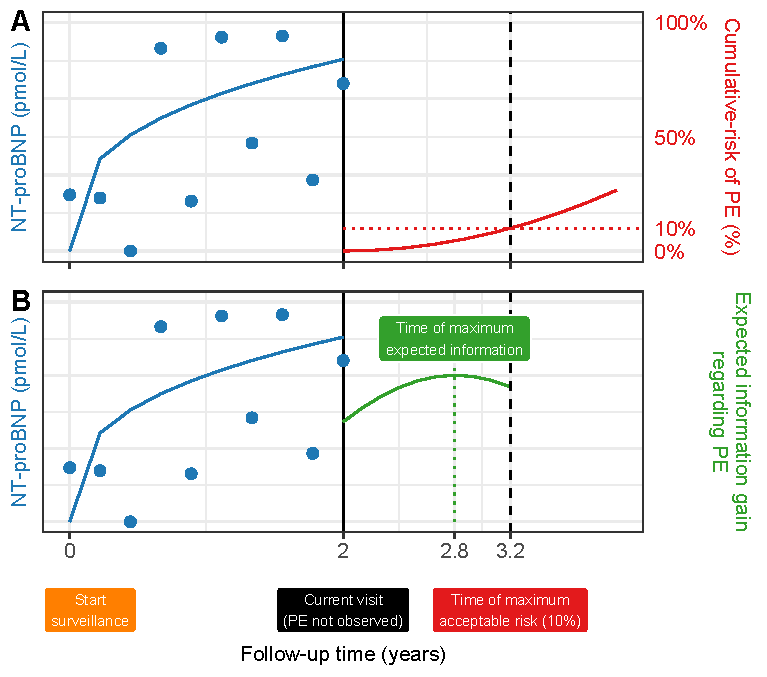
\includegraphics{contents/c6/images/c6_fig1.pdf}
\caption{\textbf{Illustration of personalized scheduling of biomarker measurements.} We plan NT-proBNP measurements until the cumulative-risk of PE (primary endpoint) at three months from the current visit is more than 10\%. \textbf{Panel~A}: Example patient with longitudinal NT-proBNP measurements and fitted profile (in blue). The time of the current visit, on which PE was not observed, is year 2. Using NT-proBNP and time of current visit data, we derive a personalized cumulative-risk profile for the patient (in red). This risk profile reaches the 10\% level at year 3.2, and hence, we are allowed to schedule new measurements until year 3.2. \textbf{Panel~B}: We calculate the expected information gain in the patient's prognosis if a new NT-proBNP measurement is done at a future time point between the current visit at year 2 and the time of the maximum acceptable risk of 10\% at year 3.2. The time of maximum expected information gain, is year 2.8, and hence, we schedule new NT-proBNP measurement at year 2.8.}
\label{c6:fig:1}
\end{figure}

\subsection{Simulation study}
After constructing the joint model and defining the thresholds needed for scheduling personalized screening visits, we proceeded to compare the personalized screening schedule to a fixed screening schedule. For the fixed schedule, we chose trimonthly intervals, in accordance with the design of the Bio-SHiFT study and daily clinical practice. Since our existing data were collected using this fixed screening schedule and hence no ‘real' data on personalized screening intervals was available, the advantages of a personalized screening design were assessed by means of a simulation study. 
We first simulated a dataset containing 750 patients. These 750 simulated patients had baseline characteristics and NT-proBNP profiles similar to the 263 patients included in the Bio-SHiFT since we simulated using the joint model fitted to the Bio-SHiFT data. We divided this data into training (700 patients), and testing (50 patients) set. For the training patients, using the joint model fitted to the Bio-SHiFT data, we generated NT-proBNP measurements at fixed follow-up time points. This schedule is similar to the schedule of the Bio-SHiFT study. We also generated a true PE time for these patients, as well as a random non-informative censoring time. Subsequently, we fitted a new joint model for these patients and, then, used this model to develop NT-proBNP measurement schedules for the test patients. To this end, in the test patients, we only generated the true PE time. Using such a design ensured that the ‘new' patients (n=50) are comparable to the ‘existing' patients (n=700) on which the model is based; if we had used the ‘real' patients (n=263 from the Bio-SHiFT study), this might not have been the case. 

Thus, for each of the 50 patients in the test set, we aimed to compare the efficacy of scheduling NT-proBNP measurements according to a fixed screening design and a personalized screening design. For the personalized screening design, the first three simulated NT-proBNP measurements were considered a given, in order to have a ‘run-in period' for the patients' longitudinal profile of NT-proBNP, since if we have a longitudinal profile available we can apply the aforementioned stepwise approach of personalized scheduling. Apart from using the risk-threshold of 7.5\% over a 3-month period, we repeated the analysis using 5\% and 10\% risk thresholds. We did so because 5\% is a lower cumulative-risk, and consequently, scheduling will stop earlier than in case of a 7.5\% risk threshold, which will give us more time to intervene with respect to the true PE time. Conversely, 10\% is a higher risk percentage than 7.5\%, and hence schedules based on the former will give us less time. 

The performance of the personalized and fixed screening schedules was compared using two outcome measures, namely, the start of the high-risk interval and the number of scheduled measurements. The high-risk interval was defined as the estimated intervention time minus the true event time (in months) (Fig. 1D). Thus, the schedule that showed a high-risk interval that was larger in absolute terms (i.e., more negative) was preferred, because such a high-risk interval enables timely intervention. In addition, assuming that the costs of NT-proBNP measurements and outpatient visits remained the same during follow-up, we prefer a procedure that requires the fewest possible repeated measurements (Supplemental Materials). All analyses were performed with R statistical software using package JMBayes~\citep{rizopoulosJMbayes}.
\section{Results}
\label{c6:sec:results}

\subsection{Baseline characteristics}
The mean age of the patients was 66.7 years, and 71.9\% were men (Table~\ref{c6:table:1}). Most patients were in NYHA class I or II (73.8\%). The median baseline NT-proBNP value was 137.3 pmol/L (IQR: 51.7-272.6). A total of 2022 NT-proBNP measurements were performed during follow-up before the PE occurred. The PE occurred in 70 patients (26.6\%). The median maximum follow-up time was 2.1~(IQR: 1.2--2.4) years.

\begin{table}
\small
\centering
\caption{\textbf{Summary of the Bio-SHiFT dataset}. The primary study endpoint (PE) was defined as the composite of cardiac death, cardiac transplantation, left ventricular assist device implantation, or hospitalization for heart failure, whichever occurred first. Abbreviations: NYHA is New York Heart Association Classification~\citep{bredy2018new}; IQR is interquartile range.}
\label{c6:table:1}
\begin{tabular}{p{8cm}r}
\toprule
\textbf{Characteristic} & Value\\
\midrule
Total patients & 263\\
\emph{PE (primary endpoint)} & 70\\
\midrule
Total NT-proBNP measurements & 2022\\
Median NT-proBNP (pg/mL) & 110.3 (IQR: 38.5--240.9)\\
Median age at inclusion (years) & 67.9 (IQR: 58.9--75.8)\\
Median BMI at inclusion & 26.5 (IQR: 24.4--30.1)\\
Median NYHA (assumed continuous) & 2 (IQR: 1--3)\\
$\mbox{Gender} = \mbox{Female}$ (\%) & 74/263 (28.1\%)\\
$\mbox{Renal failure history} = \mbox{Yes}$ (\%) & 136/263 (51.7\%)\\
$\mbox{Type-II diabetes mellitus} = \mbox{Yes}$ (\%) & 81/263 (30.8\%)\\
\midrule
Median maximum follow-up per patient (years) & 2.1 (IQR: 1.2--2.4)\\
Median \#NT-proBNP per patient & 9 (IQR: 5--10)\\
\bottomrule
\end{tabular}
\end{table}

\subsection{Association between temporal patterns of NT-proBNP and the PE}
Serially measured NT-proBNP was associated with the PE (univariable HR per doubling of NT-proBNP:~2.13, 95\%CI:~1.81--2.53, p<0.001). After adjustment for age, gender, diabetes mellitus, NYHA class, body mass index, and renal function, serially measured NT-proBNP remained independently associated with the PE (adjusted HR per doubling of NT-proBNP:~2.20, 95\%CI~:1.84--2.68, p<0.001). Two examples of dynamic risk assessment of individual patients from the Bio-SHiFT dataset based on the joint model are demonstrated in Supplemental Materials, Figure 1A-B. 

\subsection{Fixed versus personalized screening schedule: high-risk interval and number of measurements}
The median follow-up time of the 750 patients in the simulated dataset was 1.76 years~(IQR:~1.42--2.24); mean~(standard deviation) was 1.85~(0.63) years and the maximum was~3.5 years. The personalized schedule used fewer measurements as compared to the fixed (Panel~A, Figure~\ref{c6:fig:2}). The personalized schedule used a median of 7~(IQR:~7--8) and the fixed schedule, a median of~9~(IQR:~8--10) measurements. Corresponding cost estimates are demonstrated in the Supplemental Materials. The start of the high-risk intervals for the fixed and personalized screening schedules are depicted in Figure 2B. The personalized and fixed schedules showed similar results, i.e., the difference between the estimated intervention time compared to the `true' event time was a median of~6.6~(IQR:~4.5--11.3) months for the personalized and a median of~6.3~(IQR:~4.2--10.3) months for the fixed schedule (Panel~B, Figure~\ref{c6:fig:2}). In both schedules, scheduling of new sampling moments was stopped in order to undertake appropriate action, well in time before the event occurred.

\begin{figure}
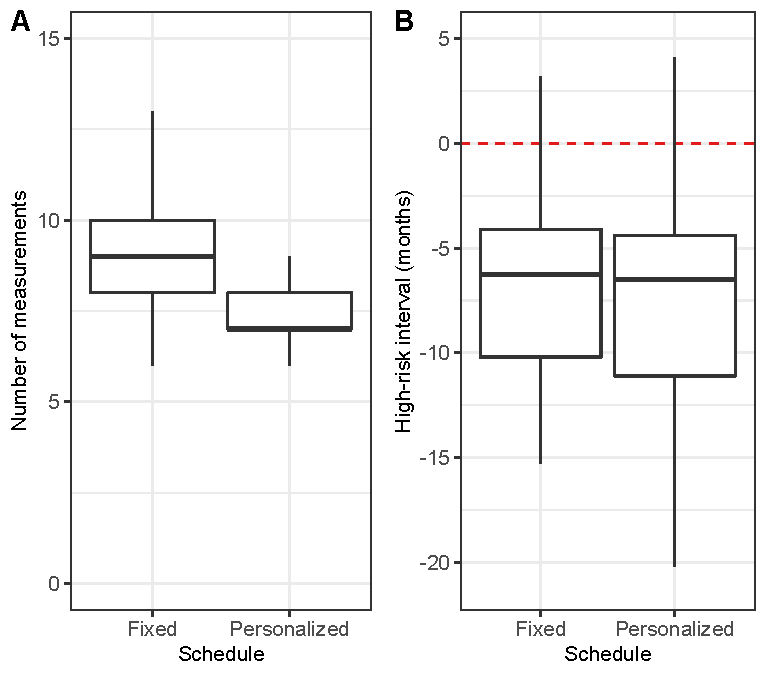
\includegraphics{contents/c6/images/c6_fig2.pdf}
\caption{\textbf{Total NT-proBNP measurements and high-risk interval (months) preceding the primary endpoint (PE)} for fixed (quarterly measurements) and personalized schedules. Results are based on a realistic simulation study of 263 test patients. NT-proBNP is measured as per personalized and fixed schedules, until a patient's cumulative-risk of obtaining PE in the subsequent three months is above 7.5\%. The boxplot for the number of measurements in Panel~A is made using data of all simulated patients. The boxplot for the high-risk interval (the difference between the time at which NT-proBNP measurements are stopped and the true simulated PE time) in Panel~B, is based on only those patients who observe PE. In Panel~B a zero high-risk interval (dashed red line) indicates that no time is available for intervention before occurrence of PE.}
\label{c6:fig:2}
\end{figure}

Results of the analyses using risk thresholds of consecutively 5\% and 10\% over three months are depicted in the Supplemental Materials, Figure~\ref{c6:fig:app1}, and Figure~\ref{c6:fig:app2}, respectively. Based on a risk threshold of 5\% over three months, the fixed and personalized screening schedules demonstrated similar results for the high-risk interval. However, again, the personalized screening schedule used fewer measurements as compared to the fixed screening schedule. The same was true for the risk threshold of 10\%. In case of a risk threshold of 5\% over three months, we found that the start of the high-risk interval was further away from the true event time as compared to a risk threshold of 7.5\% over three months. Conversely, in case of a risk threshold of 10\% over three months, the start of the high-risk interval was closer to the true event time as compared to a risk threshold of 7.5\% over three months. These results comply with the increase in the risk threshold.
\section{Discussion}
\label{c6:sec:discussion}
This study aimed to optimally schedule NT-proBNP measurements for individual patients with CHF while maximizing the gain in prognostic information and reducing costs. Furthermore, to compare the efficacy of such personalized scheduling with fixed scheduling. We found that over a median follow-up time of 1.8 years, personalized scheduling required fewer NT-proBNP measurements per patient as compared to fixed scheduling while demonstrating similar performance regarding the prevention of adverse cardiac events. Since personalized scheduling required fewer measurements, this approach is expected to reduce related health care costs as well as patient burden compared to fixed scheduling.

The findings from our study carry important implications for future trials on biomarker-guided therapy. Previous biomarker-guided trials have generally used predefined sampling intervals and target levels~\citep{khan2018does,felker2017effect}. We show that, by using a personalized approach for scheduling NT-proBNP, timely intervention is enabled while using fewer NT-proBNP measurements as compared to a fixed schedule. Even though our fixed schedule consisted of rather frequent (trimonthly) NT-pro-BNP measurements, the high-risk interval identified by the personalized schedule was similar. On top of this, the fixed schedule was outperformed by the personalized schedule in terms of the number of measurements needed per patient to obtain this result. Maximizing information gain by estimating prognosis in an individual and optimal manner, while minimizing healthcare burden, may provide novel opportunities for timely adaptation of treatment. Future trials on natriuretic peptide-guided therapy for chronic heart failure may benefit from incorporating personalized screening intervals and personalized biomarker value targets; tailoring therapeutic interventions using this approach may reveal benefits that could not be demonstrated by previous trials, by nature of their design. 

Previous studies on personalized scheduling of blood sampling moments for measurements of biomarkers of disease are scarce, but this topic seems to be gaining attention recently. Personalized scheduling has been applied to patients undergoing aortic allograft root implantation~\citep{rizopoulos2016personalized}. Similarly to our study, this study used joint modeling. Aortic gradient levels were measured according to a fixed screening schedule. The authors demonstrated that personalized scheduling of aortic gradient assessments required fewer measurements and also performed better regarding the prevention of recurrent events as compared to fixed scheduling. Recently, personalized schedules for reducing the number of biopsies in low-risk prostate cancer patients have also been developed~\citep{tomer2019personalized}. Altogether, these promising results in other disease areas concur with our conclusion that personalized screening intervals carry the potential to improve patient monitoring and to ultimately individualize and herewith improve treatment.

\subsection{Limitations}
Several aspects of this study warrant consideration. First, we made several assumptions when developing the model, defining the thresholds, and setting up of the simulation study. However, in a sensitivity analysis, we performed the simulation study for three different risk thresholds, and the results remained essentially unchanged. Second, in our investigation, we performed a so-called demonstration, meaning that the analysis was performed on one `test' set of 50 patients, and was not repeated. We performed a demonstration because we aimed to provide a proof-of-concept here. A study with multiple test sets should be performed to validate our findings further. Although, it should be noted that such repeated estimations pose a heavy computational burden. Third, we did not account for the costs of implementation. Finally, while the concept of personalized screening intervals we present here seems promising, whether it would actually lead to the prevention of adverse events remains to be investigated in a clinical trial.

\subsection{Conclusions}
In conclusion, this study demonstrates for the first time that personalized scheduling of NT-proBNP measurements in patients with CHF, as compared to fixed scheduling, shows similar performance with regard to prevention of recurrent events but requires fewer NT-proBNP measurements. If such personalized scheduling were to be applied in natriuretic peptide-guided therapy, these benefits might translate into improved outcomes. Therefore, a clinical trial incorporating personalized scheduling should be considered.
\section*{Author Contributions}
\noindent \emph{Study Design}: Akkerhuis, Umans, Boersma, Kardys\\
\noindent \emph{Data analysis}: Schuurman, Tomer\\
\noindent \emph{Drafting Manuscript}: Schuurman, Tomer\\
\noindent \emph{Analytics Strategy}: Rizopoulos, Kardys\\
\noindent \emph{Directing Implementation}: Umans, Kardys\\
\noindent \emph{Quality Control}: Kardys\\
\noindent \emph{Data Interpretation}: All authors\\
\noindent \emph{Critical revision of manuscript for important intellectual content}: All authors

\section*{Appendix}

\begin{subappendices}
\section{Details: Materials and Methods}
\subsection{Study procedures and outcome measures}
During their baseline and follow-up visits, all patients were evaluated by research physicians, who collected information on CHF-related symptoms, New York Heart Association (NYHA) class, and performed a physical examination. Information on CHF etiology, left ventricular ejection fraction, cardiovascular risk factors, medical history, and treatment was retrieved primarily from hospital records and was checked in case of ambiguities. History of cardiovascular and other comorbidities was defined as clinical diagnosis thereof reported in the hospital records.

\subsection{Blood sampling and NT-proBNP measurement}
Blood samples were processed and stored at a temperature of -80 degrees C within 2 hours after blood collection. When applicable, samples were transported to the central laboratory (Erasmus MC, Rotterdam, the Netherlands) under controlled conditions (at a temperature of -80 degrees C) until batch analysis was performed. Accordingly, results of the biomarker assays were not available to treating physicians at the time of the outpatient visits and hence did not alter patient care. Plasma NT-proBNP was analyzed using an Electrochemiluminescence immunoassay (Elecsys 2010; Roche Diagnostics, Indianapolis, IN), which measures concentrations ranging from 5 to 35000 ng/L. 

\subsection{Joint Modeling}
We utilized a joint model to estimate the association between longitudinally measured NT-proBNP and clinical outcomes. A joint model combines a linear mixed-effect (LME) model for longitudinally measured data with a Cox regression model for time-to-event data. The use of joint modeling was motivated by the following considerations. In the Bio-SHiFT study, NT-proBNP levels were measured trimonthly until the PE occurred, or until the patient was censored. Thus, naturally, patients who experienced a PE had NT-proBNP measurements available over a shorter time-course than those who did not experience a PE; or in other words, further NT-proBNP measurements could be considered as missing due to occurrence of the PE. However, commonly used methods to model such longitudinal data, for example, linear mixed-effect (LME) models, assume that missing data is non-informative with regard to a patient's health status. In other words, they do not account for the fact that patients with missing NT-proBNP values are more likely to have higher NT-proBNP levels (if hypothetically, we would have been able to observe them). This may lead to bias in the parameter estimates. In addition, a classical time-dependent Cox regression may be used in order to measure the impact of NT-proBNP on the PE. However, due to the aforementioned issue, the time-dependent Cox model may also be biased. To correctly estimate the effects, the parameters of these two types of models are required to be estimated jointly. We did so by applying the joint model.

\subsection{Costs}
Based on the number of scheduled measurements by the personalized and the fixed scheduling approach, we compared the cost estimates from the perspective of Erasmus MC as well as the perspective of society at large for both scheduling approaches. Cost estimates from the perspective of the Erasmus MC included costs of NT-proBNP sampling and measurement, as well as visiting the Cardiology outpatient clinic, at this particular institution~\citep{kanters2017update,hakkaart2015costing}. Cost estimates from the perspective of society at large included average Dutch cost estimates of NT-proBNP sampling and measurement and average Dutch cost estimates of visiting a Cardiology outpatient clinic. Moreover, patients' travel costs and patients' production losses associated with visiting the outpatient clinic were included~\citep{kanters2017update,hakkaart2015costing}.

\section{Supplemental Results}
\subsection{Fixed versus personalized screening schedule: costs}
Costs are depicted in Table~\ref{c6:table:app1}. From the perspective of the Erasmus MC, the costs associated with a visit to the Cardiology outpatient clinic, including blood sampling and NT-proBNP measurement, were €182.1 Thus, since the personalized screening schedule required two visits less than the fixed schedule (Figure~\ref{c6:fig:1}), from the perspective of the Erasmus MC the costs saved by personalized scheduling were on average €364 per patient, over a mean follow-up of 1.76 years (€207 saved per patient per year).

From the perspective of society at large, costs for visiting the outpatient clinic, blood sampling, and NT-proBNP measurement were €106.1 Travel costs and production losses amounted to €6 and €33, respectively. Altogether, costs per visit amounted to €145, with, on average, €290 saved per patient by personalized scheduling versus fixed scheduling, again over a mean follow-up of 1.76 years (€165 saved per patient per year).

In The Netherlands, the prevalence of CHF is estimated at 227,000 patients (\url{www.nivel.nl/node/4309}). In this context, personalized screening could reduce the involved annual costs by approximately €37 million from the perspective of society at large.

\begin{table}
\small
\centering
\caption{\textbf{Cost estimates from the perspective of the Erasmus MC and society at large.} Abbreviations are, CHF: chronic heart failure; NL: The Netherlands; NT-proBNP: N-terminal pro-B-type natriuretic peptide.}
\label{c6:table:app1}
\begin{tabular}{p{6cm}rr}
\toprule
\textbf{Costs} & Erasmus MC (€) & Society at large (€)\\
\midrule
NT-proBNP measurement, per measurement & 19 & 15\\
Visit to outpatient clinic, per visit & 163 & 91\\
Travel costs, per visit	& - & 6\\
Production loss costs, per visit & - & 33\\
Total costs, per visit & 182 & 145\\
\midrule	
Total costs for fixed schedule (median of 9 measurements) & 1638 & 1305\\
Total costs for personalized schedule (median of 7 measurements) & 1274 & 1015\\
Costs saved by personalized scheduling, per patient & 364 & 290\\
Annual costs saved by personalized scheduling (prevalence CHF in NL estimated at 227,000 patients) & - & 37,455,000\\
\bottomrule
\end{tabular}
\end{table}

\begin{figure}
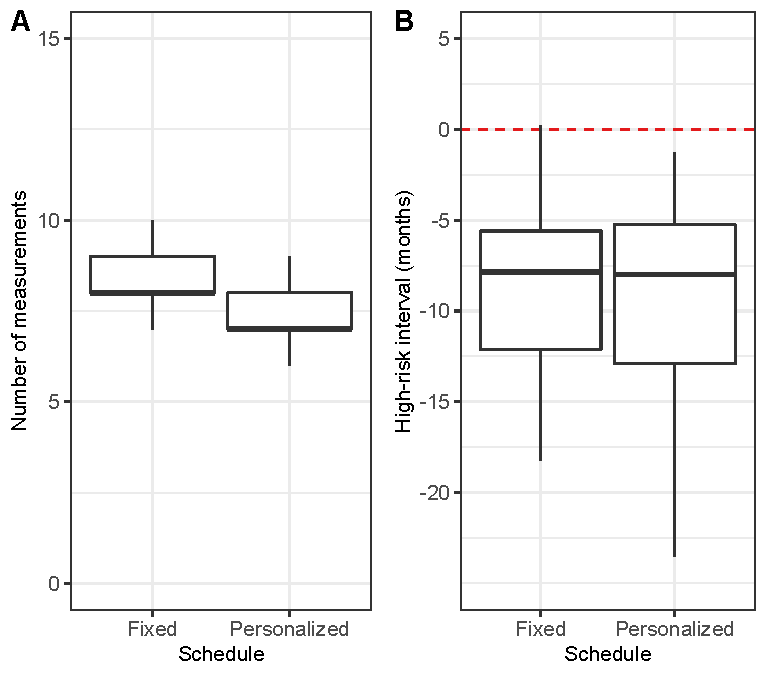
\includegraphics{contents/c6/images/c6_fig_app1.pdf}
\caption{\textbf{Total NT-proBNP measurements and high-risk interval (months) preceding the primary endpoint (PE)} for fixed (quarterly measurements) and personalized schedules. Results are based on a realistic simulation study of 263 test patients. NT-proBNP is measured as per personalized and fixed schedules, until a patient's cumulative-risk of obtaining PE in the subsequent three months is above 5\%. The boxplot for the number of measurements in Panel~A is made using data of all simulated patients. The boxplot for the high-risk interval (the difference between the time at which NT-proBNP measurements are stopped and the true simulated PE time) in Panel~B, is based on only those patients who observe PE. In Panel~B a zero high-risk interval (dashed red line) indicates that no time is available for intervention before occurrence of PE.}
\label{c6:fig:app1}
\end{figure}

\begin{figure}
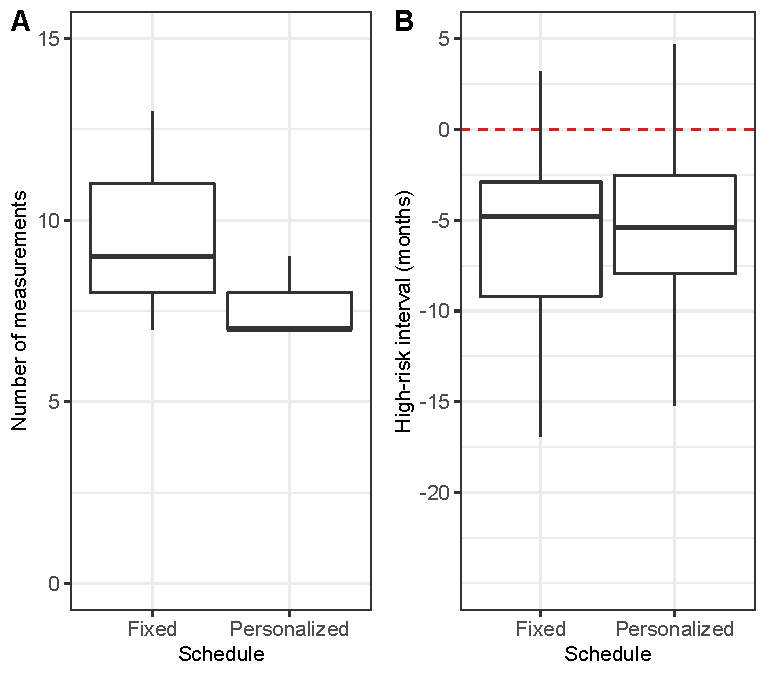
\includegraphics{contents/c6/images/c6_fig_app2.pdf}
\caption{\textbf{Total NT-proBNP measurements and high-risk interval (months) preceding the primary endpoint (PE)} for fixed (quarterly measurements) and personalized schedules. Results are based on a realistic simulation study of 263 test patients. NT-proBNP is measured as per personalized and fixed schedules, until a patient's cumulative-risk of obtaining PE in the subsequent three months is above 10\%. The boxplot for the number of measurements in Panel~A is made using data of all simulated patients. The boxplot for the high-risk interval (the difference between the time at which NT-proBNP measurements are stopped and the true simulated PE time) in Panel~B, is based on only those patients who observe PE. In Panel~B a zero high-risk interval (dashed red line) indicates that no time is available for intervention before occurrence of PE.}
\label{c6:fig:app2}
\end{figure}
\end{subappendices}

\clearpage
\bibliographystyle{apalike}
\bibliography{c6_bib}